Detached from a noise model, the goal of image restoration is to estimate the true image $Y$ from an incomplete or corrupted (noisy) observation $X$. Let $\mathbf{i} = [i_1, i_2, \dots, i_d]^T$ be a column vector that defines the coordinates of each voxel in a \textit{d}-dimensional image space. Then $x_{\mathbf{i}}$ and $y_{\mathbf{i}}$ represent the incomplete observation and the corresponding true image value at voxel $\mathbf{i}$, respectively; and the entire image can be represented as $X = [x_{\mathbf{i}}]$ and $Y = [y_{\mathbf{i}}]$, respectively.

In the most general form, the observation model can be defined as $X$ being a mapping of $Y$ through a function $\mathcal{F}$:
\begin{equation}\label{eq:observation-model}
    X = \mathcal{F} (Y)
\end{equation}
 And the function $\mathcal{F}$ can vary depending on the noise model (e.g., additive or multiplicative noise, etc.).

This mapping, however, is not injective and therefore, the inverse problem\footnote{Referred to as image restoration, reconstruction or denoising} to estimate $Y$ from $X$, is an \textit{ill-posed} problem, meaning that there are multiple possible solutions for $Y$ that could generate $X$.

Image restoration techniques have been explored in both the spatial and transform domains. In the spatial domain, several linear and nonlinear filtering techniques exist, utilizing different kernels to perform direct manipulation on pixel values. Linear filters, such as the mean filter, compute the average of pixel values in a neighborhood and, in doing so, smooth the image but usually result in edge blurring.

Non-linear filters, like the median filter, replace each pixel with the median value of its neighbors and are much better at removing salt-and-pepper noise. Wiener filtering is another example, operating on statistical principles. The mean squared error between the estimated and true image is minimized; that is, the filter response is adjusted against the local image variance. This makes Wiener filtering particularly effective for Gaussian noise, as it may adaptively filter based on the estimated noise level and characteristics of the signal and often results in better denoising performance compared to linear methods. Other non-linear approaches, such as bilateral filtering, combine spatial proximity and intensity similarity, allowing for selective smoothing that  preserves sharpness around edges. 

Besides these filtering techniques, many algorithms make great use of prior knowledge about image characteristics. Standard priors might include sparsity, smoothness, and texture assumptions. For instance, the model of TV denoising assumes natural images are piece-wise smooth, allowing the algorithm to preserve edges while smoothing out flat regions. This method minimizes the global intensity variation of the image, resulting in a denoised image preserving important structural information.

The principle behind \gls{NLM} denoising also builds on the redundancy of similar patches in the image and estimates a pixel value by taking a weighted average over other pixels with a similar local structure, regardless of their spatial distance. By utilizing these priors, denoising algorithms can indeed aggressively use the intrinsic properties of the images and thereby enhance the visual quality and provide estimates closer to the true image.

A lot of the mentioned algorithm assume the noise prior to be additive. This can be written as:
\begin{equation}
    X = Y + N
\end{equation}
and many more assume the noise to be \gls{AWGN} with noise of form in \cref{eq:awgn}. This is because the normal distribution has nice mathematical properties, allowing to derive theoretical guarantees.

\begin{equation}\label{eq:awgn}
    N \sim \mathcal{N}(0, \sigma^2)
\end{equation}

In the following, we shall look at one such \gls{AWGN} denoising algorithm--the celebrated \gls{BM3D} algorithm, introduced first by \citeauthor{dabovImageDenoisingSparse2007} in \cite{dabovImageDenoisingSparse2007}, building upon many of the classical denoising techniques such as the transform domain denoising, non-local means and filtering methods (such as the Wiener filter). We will look at its application to the \gls{MPES} data, by first defining a noise model for the data, discussing the Anscombe \gls{VST}, finding optimal denoising level for different noise levels and evaluating its performance using the \gls{MSSSIM} metric.

\section{BM3D: Denoising in Sparse Domain}
As shown in \cref{alg:bm3d}, the \gls{BM3D} scheme works by grouping similar patches in a 2D image and applying a 3D transform\footnote{This algorithm has also been proposed for 3D images, dubbed BM4D.}. This leads to an enhanced sparse representation of the image which after filtering is transformed back to the spatial domain.
% Main BM3D Algorithm
\begin{algorithm}
    \caption{BM3D Denoising Algorithm}\label{alg:bm3d}
    \begin{algorithmic}[1]
    \Require Noisy image $X$
    \Ensure Denoised image $X_h$
    \Statex
    \Procedure{BM3D}{$X$, $\sigma^2$}
        \State $X_h \gets I$
        
        \For{each reference block $B_r$ in $X$}
            \State $B \gets \textsc{Grouping}(B_r)$
            \State $B_{\text{filtered}} \gets \textsc{CollaborativeFiltering}(B)$
            \State Aggregate $B_{\text{filtered}}$ into $X_h$
        \EndFor
        
        \State \textbf{return} $X_h$
    \EndProcedure
    \end{algorithmic}
\end{algorithm}

In the Grouping step, blocks which are the least dissimilar to a reference block $B_r$ are grouped together. The dissimilarity measure used is the $l^2$-distance. The Collaborative Filtering\footnote{Interestingly, collaborative filtering has been the backbone of recommendation systems such as by Netflix and Spotify.} shown in \cref{alg:collaborativefiltering} is then applied to the grouped blocks. This step consists of a 3D transform such as the discrete cosine transform (or the wavelet transform can be used). A filter is applied to the transformed blocks to remove noise, initially by hard thresholding and in the second run by Wiener filtering. The inverse 3D transform is then applied to the filtered blocks, and the filtered blocks are aggregated to form the estimate. The first run is considered the basic estimate, and it is only after Collaborative Wiener filtering that the final estimate is obtained.
    
% Collaborative Filtering Algorithm
\begin{algorithm}
    \caption{Collaborative Filtering}\label{alg:collaborativefiltering}
    \begin{algorithmic}[1]
    \Require Group of similar blocks $B$
    \Ensure Filtered block $B_{\text{filtered}}$
    \Procedure{CollaborativeFiltering}{$B$}
        \State $B_{\text{transformed}} \gets \textsc{3DTransform}(B)$
        \State $B_{\text{filtered}} \gets \textsc{ApplyFiltering}(B_{\text{transformed}})$ \Comment{Hard thresholding or Wiener filter}
        \State $B_{\text{inverse}} \gets \textsc{Inverse3DTransform}(B_{\text{filtered}})$
        \State Aggregate $B_{\text{inverse}}$ into $B_{\text{filtered}}$
        \State \textbf{return} $B_{\text{filtered}}$
    \EndProcedure
    \end{algorithmic}
\end{algorithm}

The \gls{BM3D} algorithm had showed one of the best denoising performances and can only be contested by the recent deep-learning based denoising methods. 

\section{Poisson Noise Model}\label{sec:poisson-noise-model}

\begin{figure}
    \centering

    \begin{subfigure}[b]{1\linewidth}
        \centering
        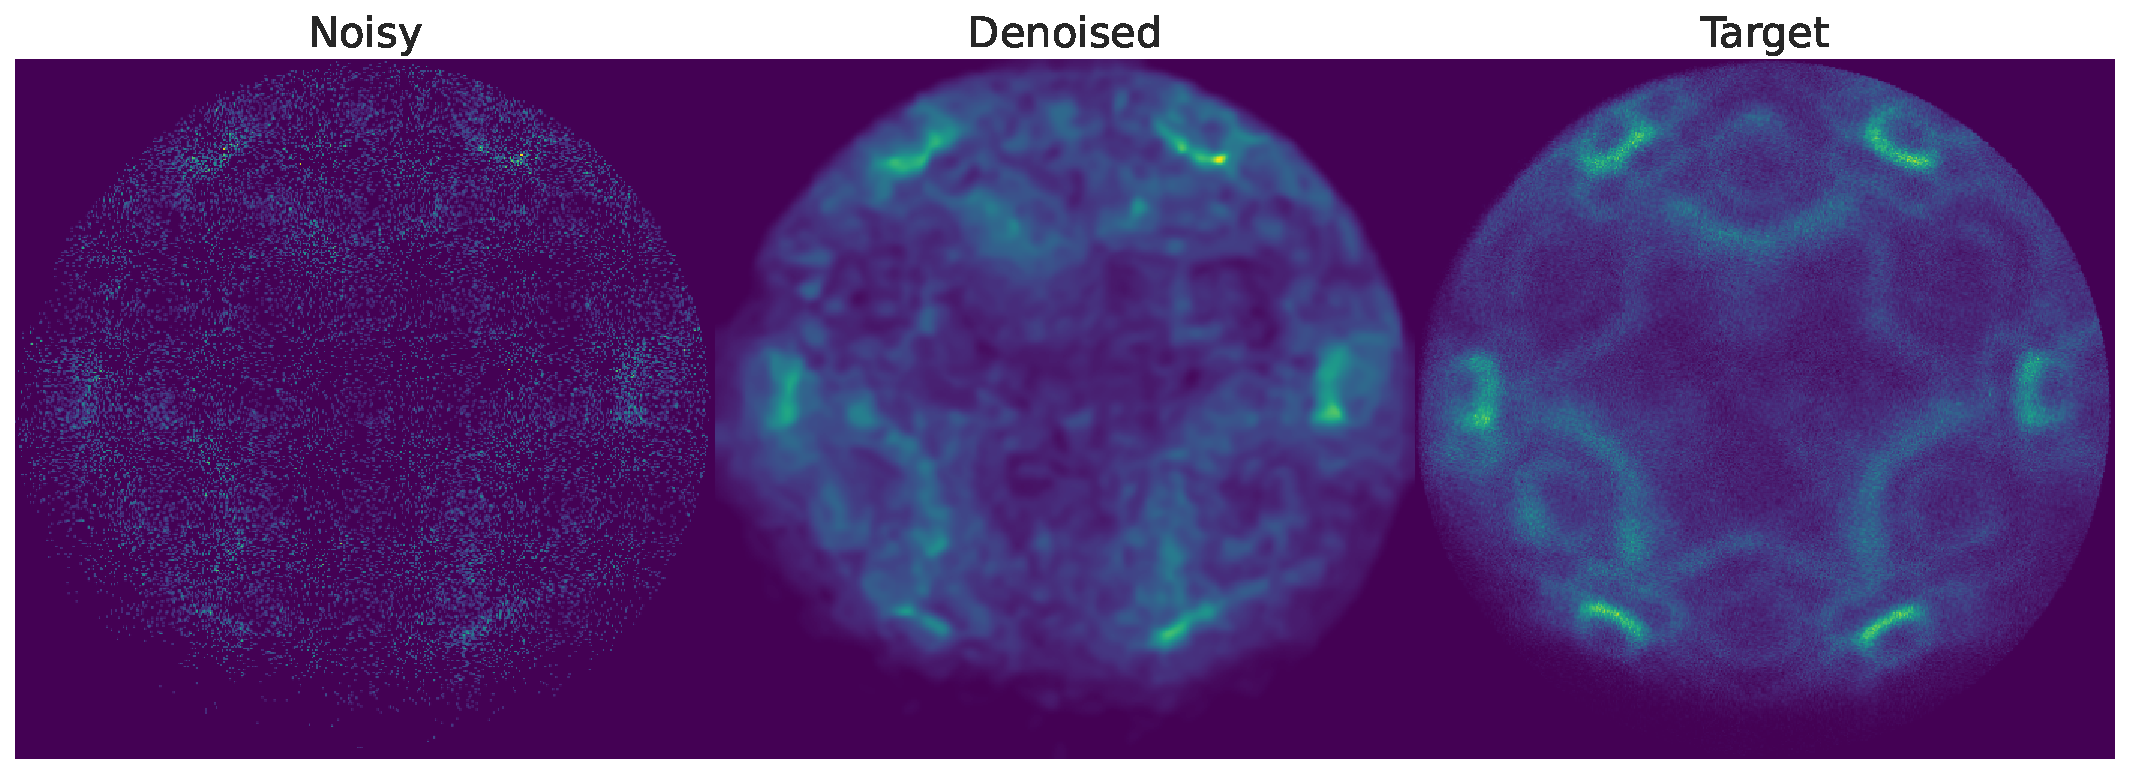
\includegraphics[width=1\linewidth]{images/noisy_denoised_ref_2M_avg_bm3d.pdf}
        \caption{\num{2e6} count dataset. The denoising performance is quite poor, even with the adjusted optimal $\sigma_{\text{o}}\approx0.4$.}
        \label{fig:noisy-denoised-ref-2M-avg-bm3d}
    \end{subfigure}

    \begin{subfigure}[b]{1\linewidth}
        \centering
        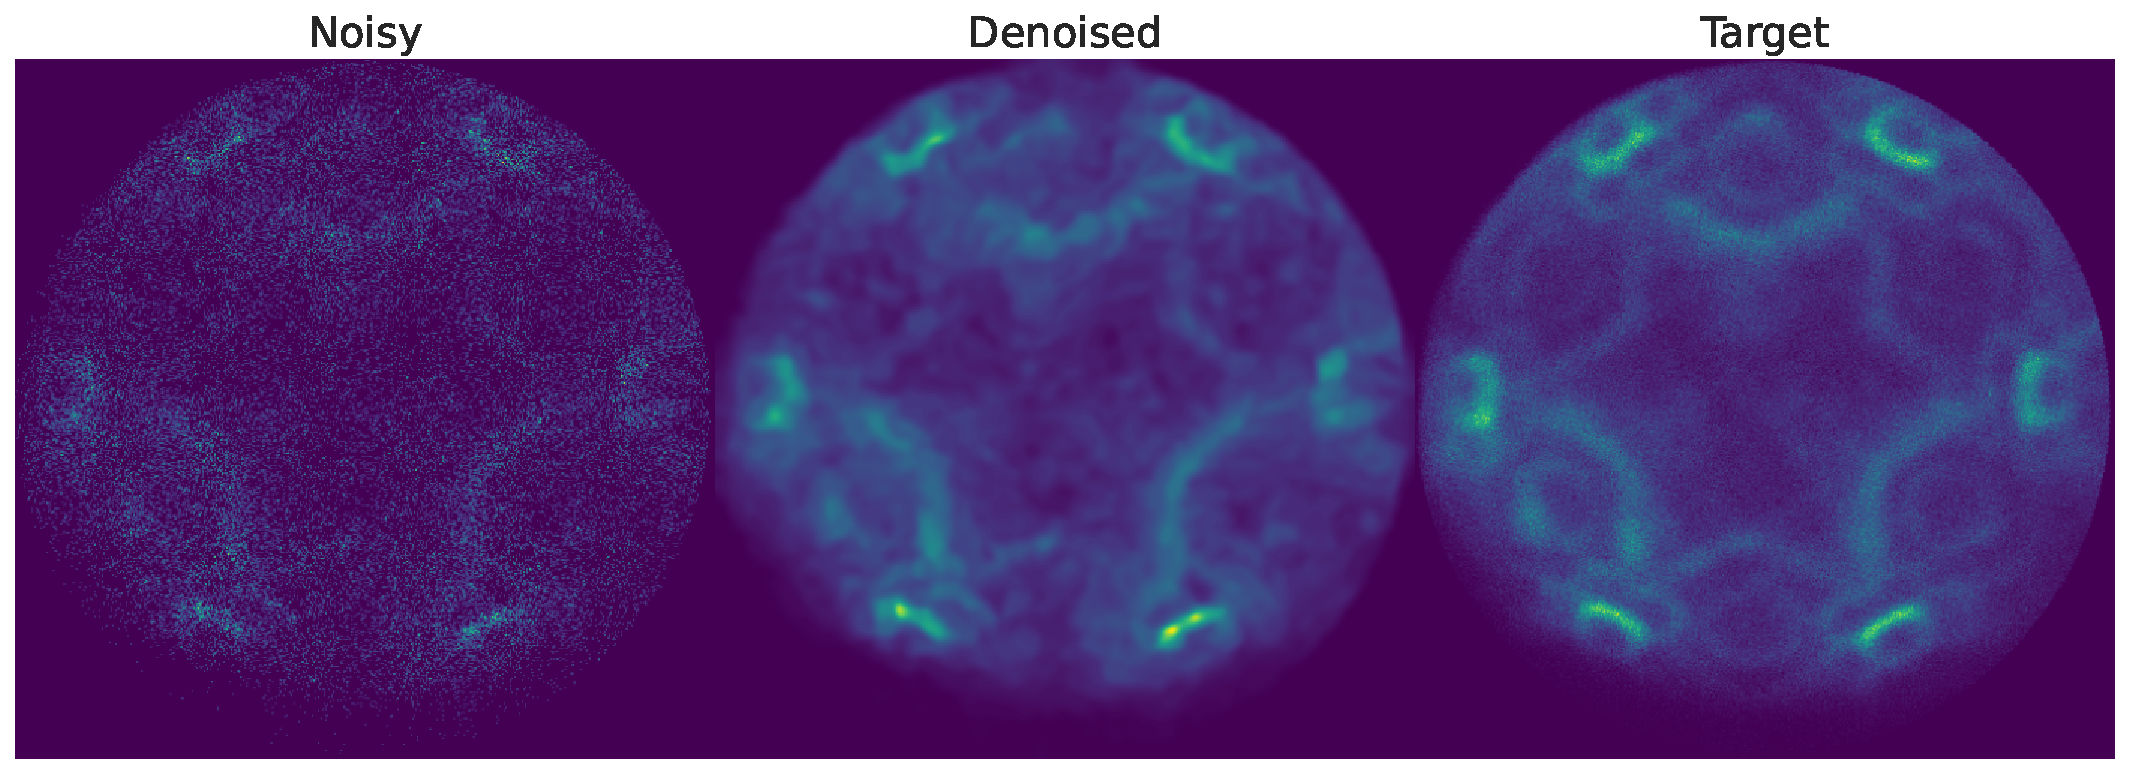
\includegraphics[width=1\linewidth]{images/noisy_denoised_ref_4M_avg_bm3d.pdf}
        \caption{\num{4e6} count dataset. The denoising performance leaves room for improvement, using the adjusted optimal $\sigma_{\text{o}}\approx0.4$.}
        \label{fig:noisy-denoised-ref-4M-avg-bm3d}
    \end{subfigure}

    \begin{subfigure}[b]{1\linewidth}
        \centering
        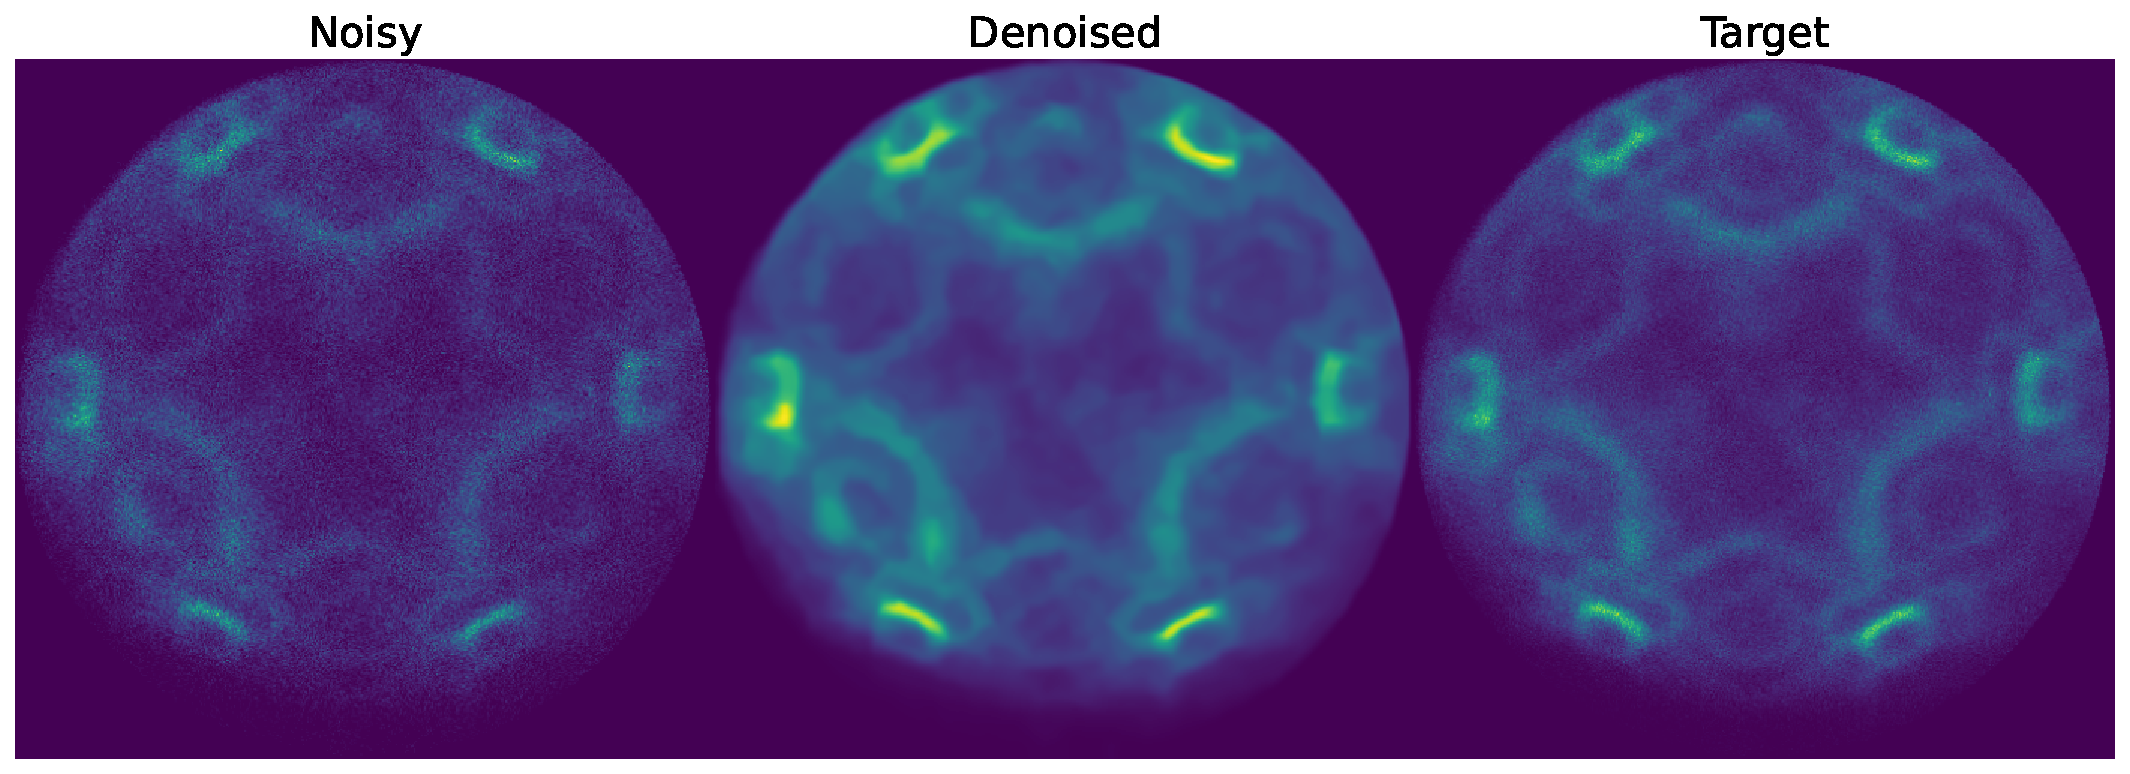
\includegraphics[width=1\linewidth]{images/noisy_denoised_ref_48M_avg_bm3d.pdf}
        \caption{\num{4.8e7} count dataset. At this count rate, \gls{MSSSIM} reports lower values for the denoised images compared to the noisy images, even though the denoised image features are well-preserved.}
        \label{fig:noisy-denoised-ref-48M-avg-bm3d}
    \end{subfigure}

    \caption{Comparison of noisy, denoised, and target images for different count datasets, where the noisy and target images were formed using window-averaging over \num{10} \gls{E} slices to form \gls{ky}-\gls{kx} images. The \gls{BM3D} algorithm with Anscombe transform (\cref{alg:anscombe-bm3d}) is applied to counts of \num{2e6}, \num{4e6}, and \num{4.8e7}.}
    \label{fig:combined-noisy-denoised}
\end{figure}

For low count settings, the observed intensity $x_{\mathbf{i}} \in \mathbb{Z}_{\geq 0}$ at each voxel (with $\mathbf{i} = [i_1, i_2, \dots, i_d]^T$ the coordinate vector in $d$-dimensional space) can be modeled as an independent Poisson \gls{rv} with parameter $y_{\mathbf{i}}$--the true intensity \cite{makitaloOptimalInversionAnscombe2011,kimDeepLearningbasedStatistical2021}. This is shown in \cref{section:photoelectron-counting-stats} to be true for a constant intensity light source. The relation can be expressed as: $x_{\mathbf{i}} \sim \text{Poi}(y_{\mathbf{i}})$

\begin{equation}
    P(x_{\mathbf{i}} = x| y_{\mathbf{i}} = y) = \frac{y^x e^{-y}}{x!}
\end{equation}


Here, $x$ represents the observation at voxel $X$, while $y$ corresponds to the expected number of detected electrons, the underlying intensity that we aim to recover. Formally $\mathbb{E}[x_{\mathbf{i}} | y_{\mathbf{i}}] = y_{\mathbf{i}}$

The Poisson noise can then be written as:
\begin{equation}
    N_{\mathbf{i}} = x_{\mathbf{i}} - \mathbb{E}[x_{\mathbf{i}} | y_{\mathbf{i}}]
\end{equation}

This noise is signal dependent as the variance is dependent on the true signal $Var[N_{\mathbf{i}} | y_{\mathbf{i}}] = [x_{\mathbf{i}} | y_{\mathbf{i}}] = y_{\mathbf{i}}$ and hence it can be seen that the with decreasing intensity, the noise increases.

\section{Variance Stabilization Transform: Anscombe}

\Glspl{VST} are used to map the values of the data to a new domain so that the variance becomes constant. \citeauthor{anscombeTransformationPoissonBinomial1948} \cite{anscombeTransformationPoissonBinomial1948} introduced such a \gls{VST} for data distributed according to the Poisson, Binomial, and Negative Binomial distributions. The Anscombe transform for the Poisson distribution is defined as:
\begin{equation}
    T(Z) = 2 \sqrt{Z + \frac{3}{8}}
\end{equation}

Applying this transformation to a Poisson distributed \gls{rv} maps the data such that the variance becomes approximately constant. $T(Z)$ can then be denoised using \gls{AWGN} denoising techniques such as \gls{BM3D}. 
The denoised signal $\mathbb{Z}$ as is an estimate of expected value of $T(Z)$ conditioned on the true signal $Y$ we aim to recover.
\begin{equation}
    \mathbb{Z} = \mathbb{E}[T(Z) | Y]
\end{equation}
Hence, the final estimate for the true signal $Y$ can be obtained by applying the inverse Anscombe transform to $\mathbb{Z}$.
\begin{equation}
    \hat{Y} = T^{-1}(\mathbb{Z}) = \mathbb{E}[Z | T(Z) = \mathbb{Z}]
\end{equation}
Since the transformation is non-linear, an algebraic inverse is asymptotically biased. \citeauthor{makitaloOptimalInversionAnscombe2011} \cite{makitaloOptimalInversionAnscombe2011} proposed an exact unbiased inverse of $\mathbb{Z}$ giving the denoised estimate $\hat{Y}$. This method performs better than methods based on explicit Poisson noise removal. Therefore, in the next few sections we make use of the scheme described in \cref{alg:anscombe-bm3d} to denoise 2D image slices from the \gls{MPES} data.

\begin{algorithm}
    \caption{Algorithm to Denoise Poisson Corrupted Images}\label{alg:anscombe-bm3d}
    \begin{algorithmic}[1]
    \Require Noisy image $X$
    \Ensure Denoised image $X_h$
    \Statex
    \Procedure{AnscombeBM3D}{$X$, $\sigma^2$}
        \State $X_{\text{anscombe}} \gets \textsc{AnscombeTransform}(I)$
        
        \State $X_{\text{bm3d}} \gets \textsc{BM3D}(I_{\text{anscombe}}, \sigma^2, b, Y, \tau)$
        
        \State $X_h \gets \textsc{InverseAnscombeTransform}(I_{\text{bm3d}})$
        
        \State \textbf{return} $X_h$
    \EndProcedure
    \end{algorithmic}
\end{algorithm}

\section{Denoising MPES data}
As described in \cref{section:datasets}, a 3D image is constructed by binning over the three physical axes $k_x$, $k_y$, $E$ from different datasets. By slicing along these axes, different 2D images can be generated for analysis. We evaluate the \gls{BM3D} algorithm, with and without the Anscombe transform, using the \gls{GrIr} dataset, which has the highest average counts of all datasets. Despite this, the average voxel intensity is low, making a true, noise-free image unavailable. This limitation complicates the task of evaluating denoising performance, as standard metrics rely on comparison with such a noise-free reference.

\Gls{IQA} is a field dedicated to measuring the objective and perpetual quality of an image. Objective metrics such as \gls{PSNR}, \gls{SSIM}, \gls{MSE} and \gls{MSSSIM} require a reference image---the true image---to compare the denoised image against. No-reference metrics also exist, such as \gls{NIQE}. However, these metrics are designed for real-world, non-scientific images. Subjective metrics such as the \gls{MOS} can also be used, but these require evaluations by a group of experts, which can be impractical.

\begin{figure}
    \centering
    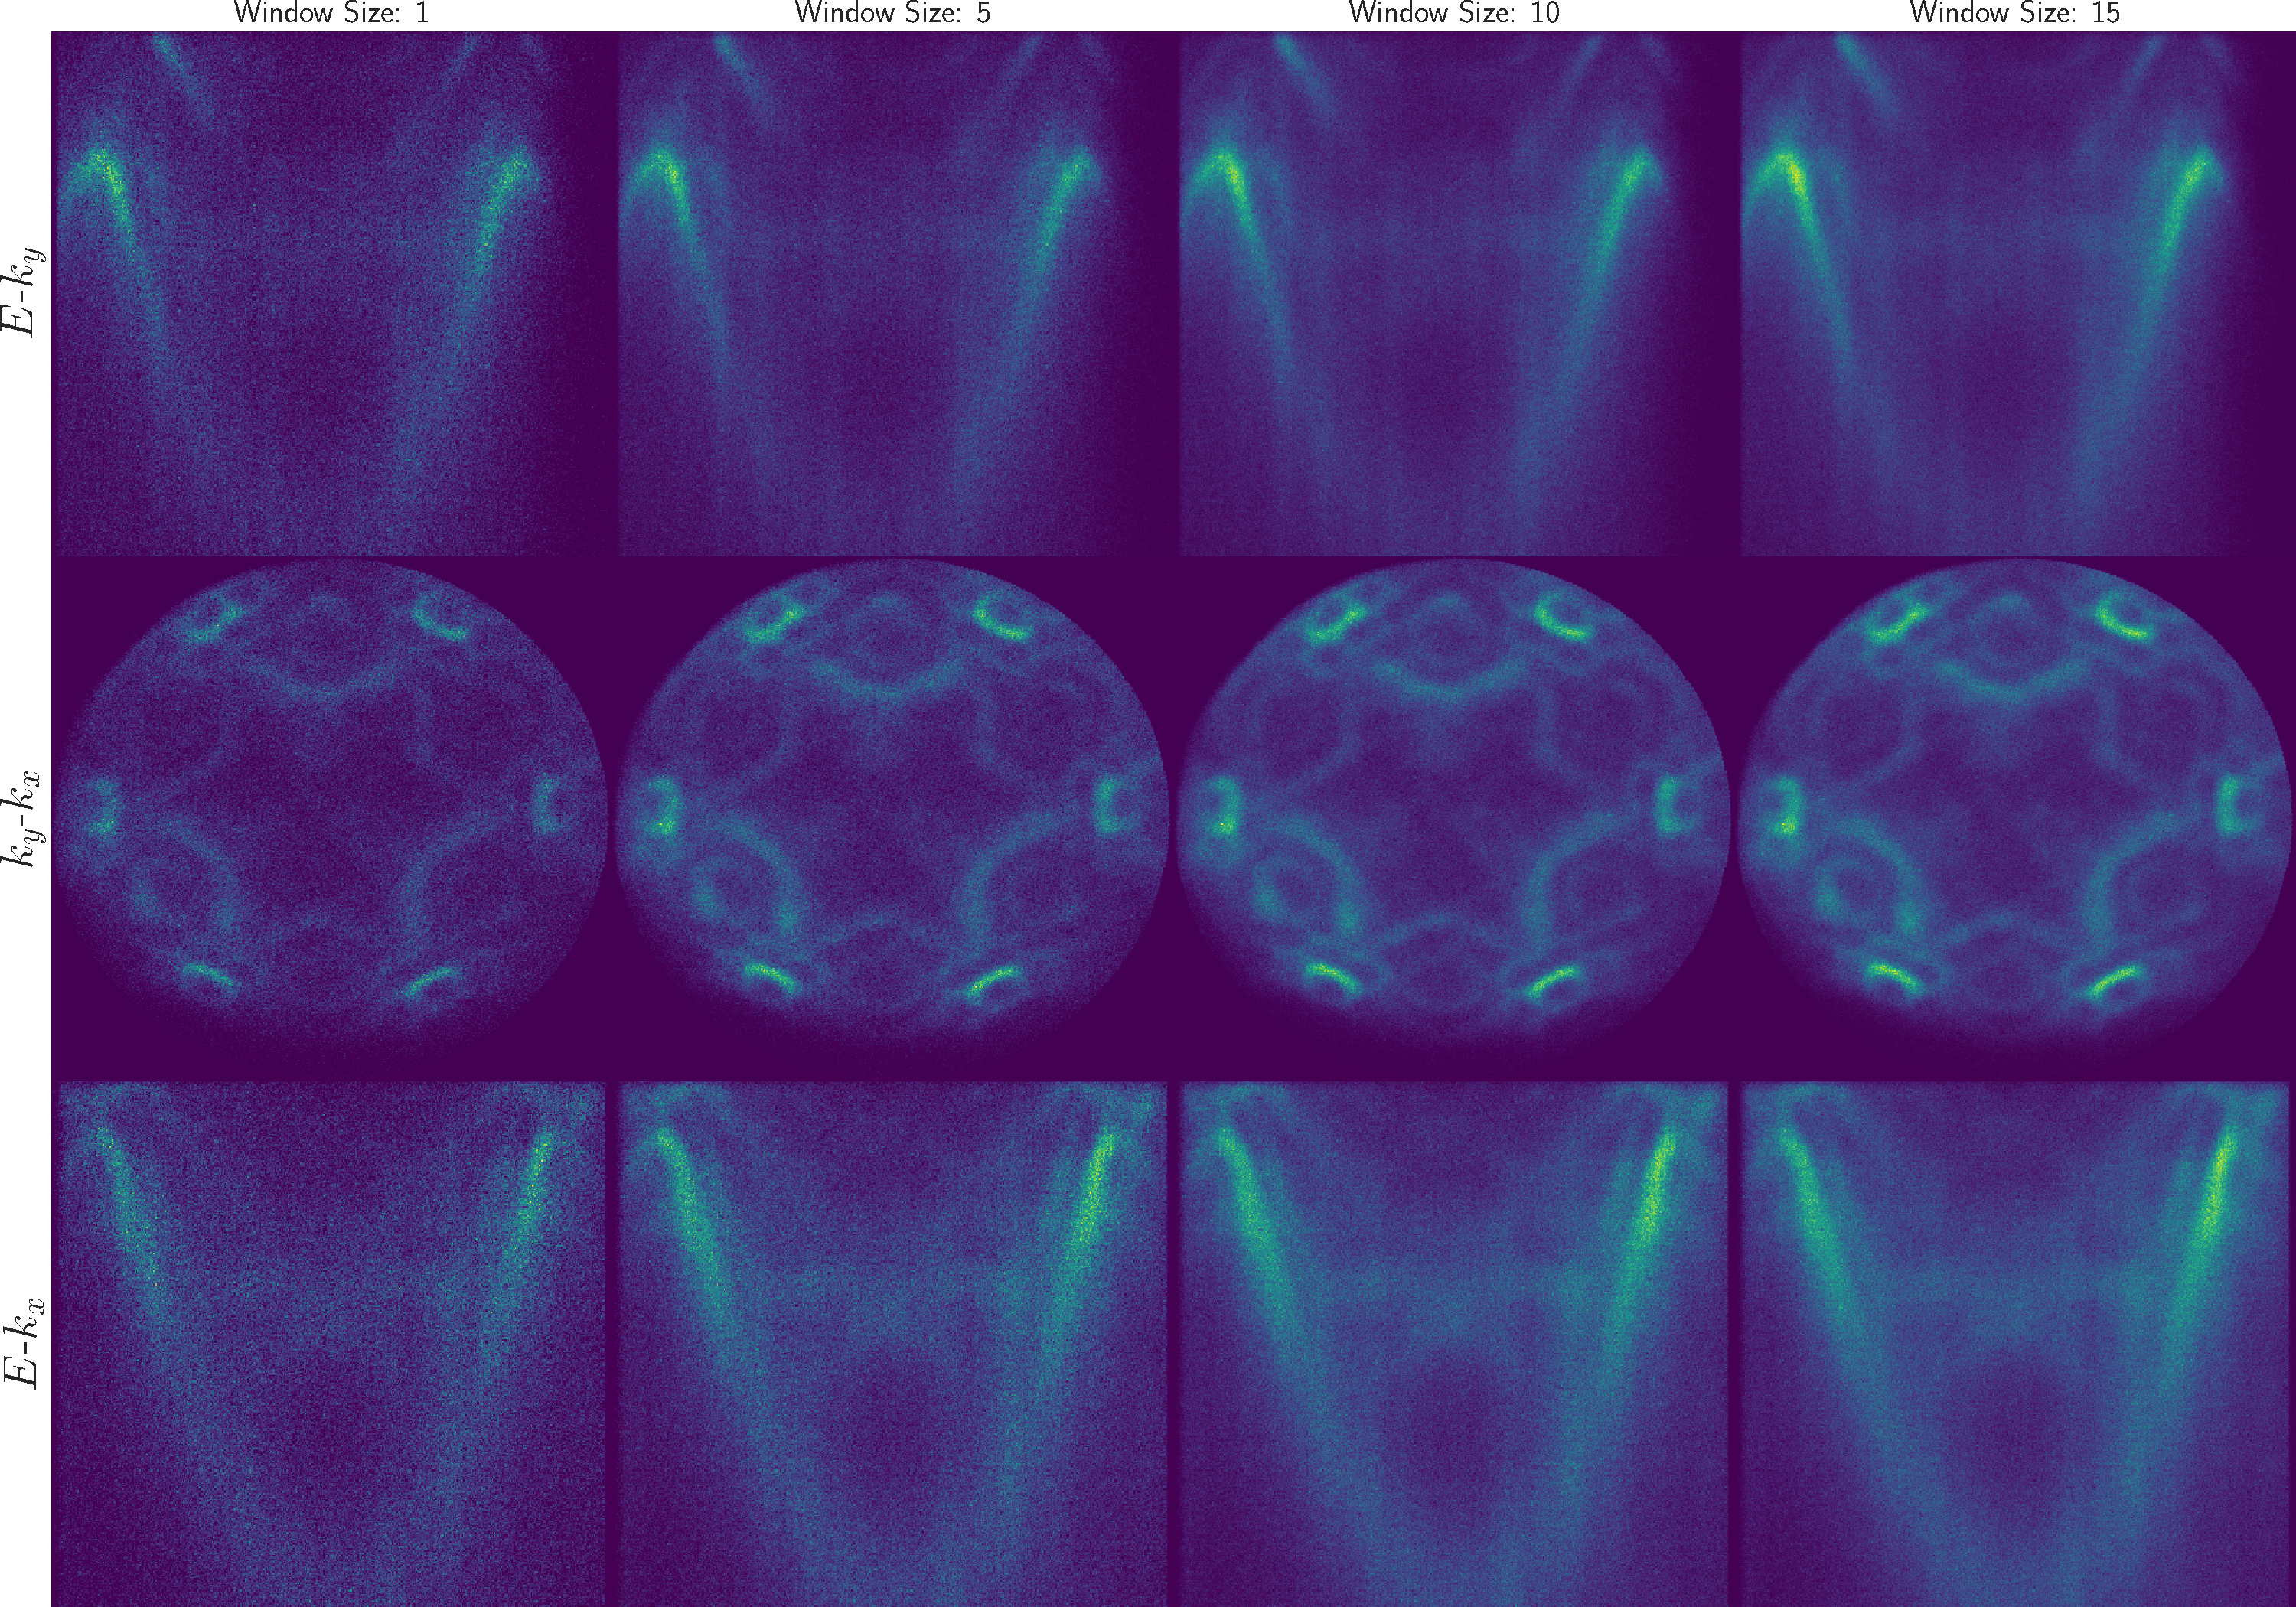
\includegraphics[width=1\linewidth]{images/slices.pdf}
    \caption{$E$, $k_y$, and $k_x$ slices at arbitrary positions of the \gls{GrIr} 3D dataset, showing the effect of averaging across different window sizes. The leftmost column shows a single slice with significant noise, while subsequent columns show window-averaged images of 5, 10, and 15 slices. Increasing the window size progressively reduces noise, at the cost of feature broadening. This trade-off highlights the difficulty in obtaining a true, noise-free reference image even through averaging techniques.}
    \label{fig:slices}
\end{figure}

Given the low counts in the dataset, a possible method to create a higher quality reference image is to perform window-average across neighboring slices. \cref{fig:slices} illustrates such a case, where noise is progressively reduced by averaging across windows of increasing size (see \cref{fig:3d-gr-ir} for a 3D depiction of slice axis), at the cost of feature blurring. Even with a large window size, an ideal, noise-free reference image is not obtainable.

To address this, we assess metrics that are more resilient to noisy reference images. In \cref{sec:metric_comparison_experiment}, we compare the performance of different metrics (\gls{PSNR}, \gls{SSIM}, \gls{MSE} and \gls{MSSSIM}) for evaluating the denoising performance. Our findings suggest that the \gls{MSSSIM} metric is particularly well-suited for evaluating the denoising performance of images, when comparing against a noisy reference image. The \gls{MSSSIM} metric, conceived by \citeauthor{wangMultiscaleStructuralSimilarity2003} \cite{wangMultiscaleStructuralSimilarity2003}, extends SSIM by incorporating multiple scales. 

Given that the ideal denoising aims to produce distortion-free images, one free from artifacts and removing all unwanted signal, it makes sense to target structural similarity rather than relative intensity values against the reference. Hence, throughout this study, the images are normalized to the [\num{0}, \num{1}] range. This normalization ensures that comparisons focus on relative differences in image structures and features, rather than on absolute intensity values.

\subsection{Denoising Evaluation: Single and Window-Averaged Images}
Let us start with attempting to denoise the noisy realization with \num{1.6e7} electron counts ($\approx$ \qty{2}{h} of acquisition) of the $k_y$-$k_x$ images shown in \cref{fig:slices}, as the target has clear features to compare against. We use the Anscombe--\gls{BM3D}--Inverse Anscombe scheme described in \cref{alg:anscombe-bm3d}. Single slice and window-averaged images \numlist{1;5;10;15} are compared against the reference (single slice and window-averaged of the \num{1.86e8} counts dataset) using the \gls{MSSSIM} metric.

\begin{figure}
    \centering
    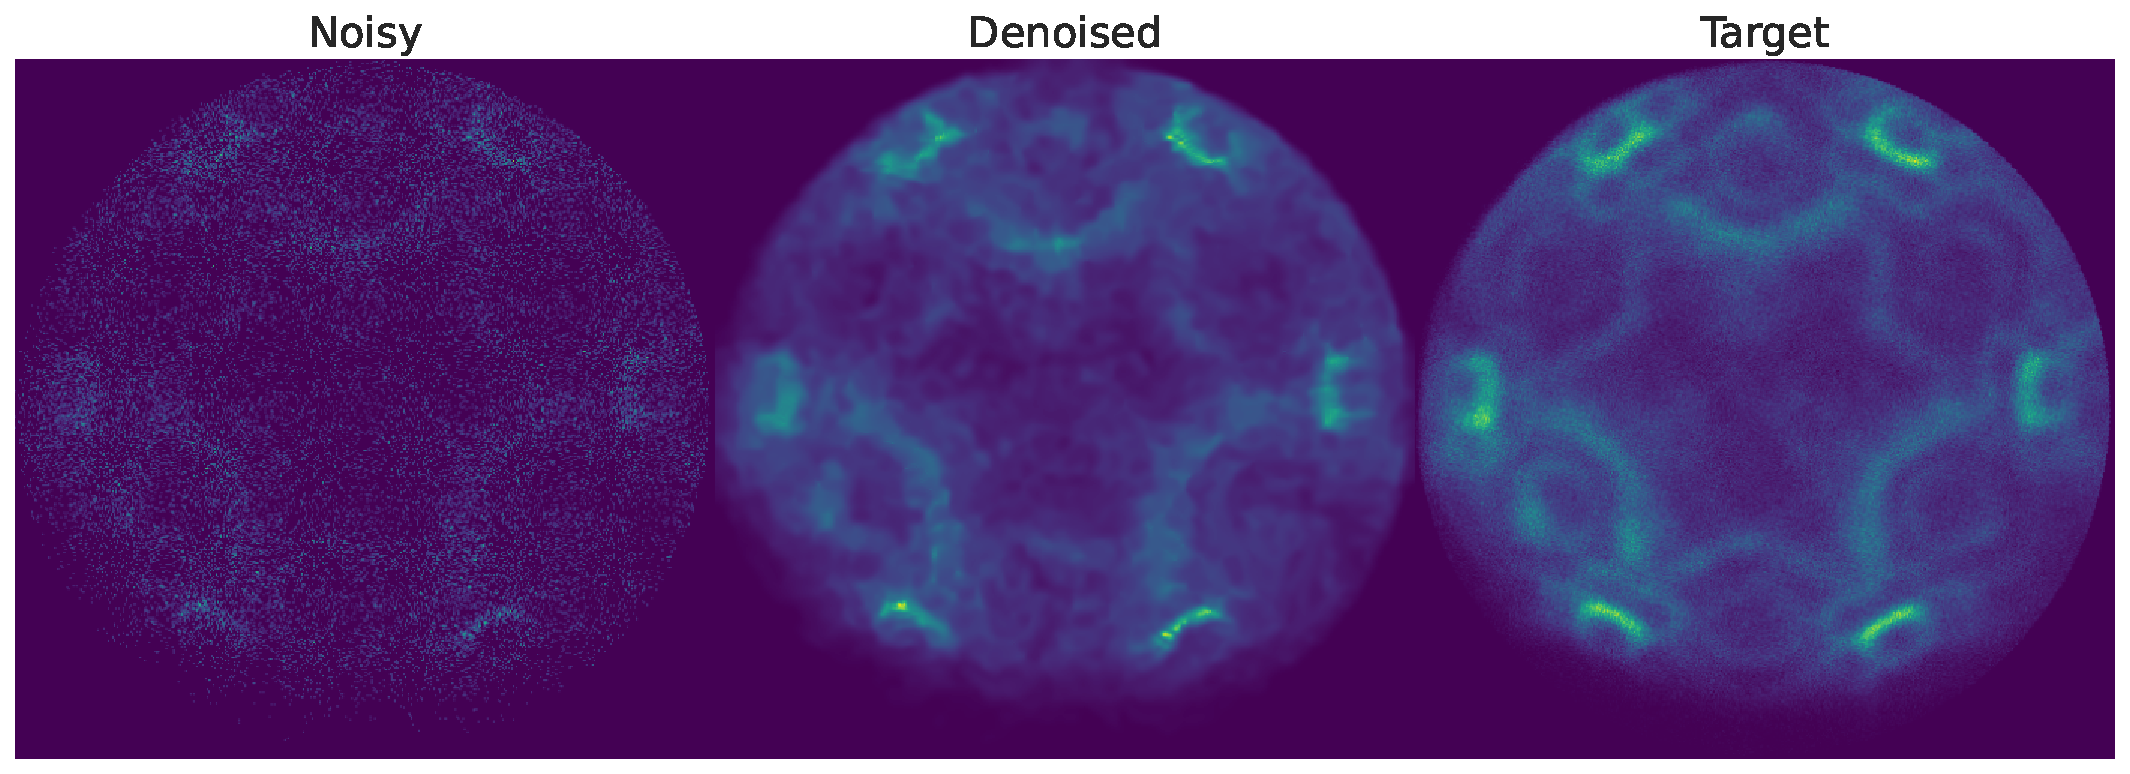
\includegraphics[width=1\linewidth]{images/noisy_denoised_ref_16M_avg_bm3d.pdf}
    \caption{Noisy, denoised, and target images. The noisy image is window-average of 5 slices along the $E$ dimension, and the target image the window-average of 15 slices.}
    \label{fig:noisy-denoised-ref-16M-avg-bm3d}
\end{figure}

\cref{fig:confusion_matrix_msssim_window_avg} presents a confusion matrix that shows how the metric varies with different window sizes.  It becomes evident that a larger window size yields a better comparison for denoising. This is because the larger window size reduces the noise in the target image, leading to a more accurate evaluation. One example of noisy, denoised, and target images is shown in \cref{fig:noisy-denoised-ref-16M-avg-bm3d}, with the noisy image formed by window-averaging 5 slices along the $E$ axis and the target image formed by window-averaging 15 slices. 

\begin{figure}
    \centering
    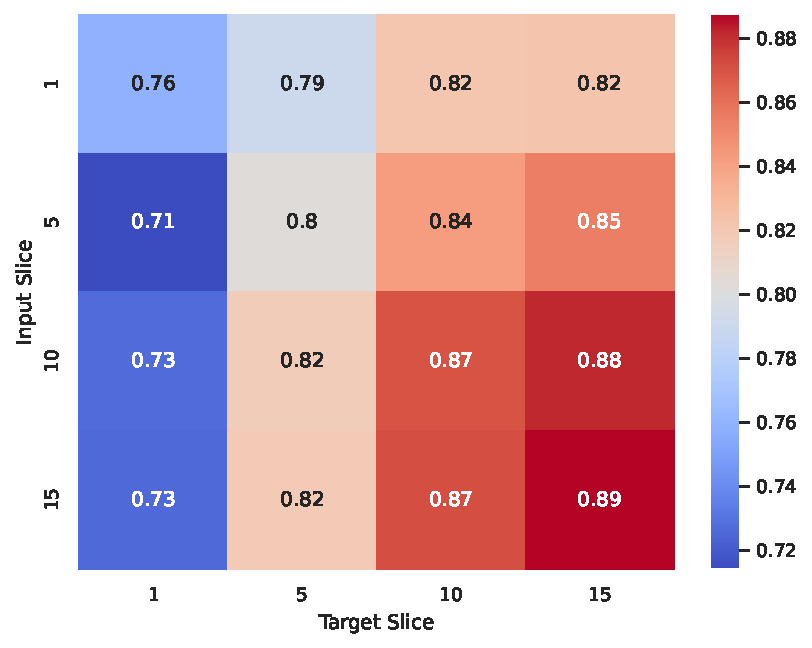
\includegraphics[width=0.5\linewidth]{images/confusion_matrix_msssim_window_avg.pdf}
    \caption{Confusion matrix showing the \gls{MSSSIM} values for different window-averaged input and target images. The \gls{MSSSIM} is computed for the denoised images using \cref{alg:anscombe-bm3d}. The matrix shows that using a larger window for target image leads to better comparison of denoising.}
    \label{fig:confusion_matrix_msssim_window_avg}
\end{figure}

\subsection{Finding the Optimal Sigma}
\begin{figure}
    \centering
    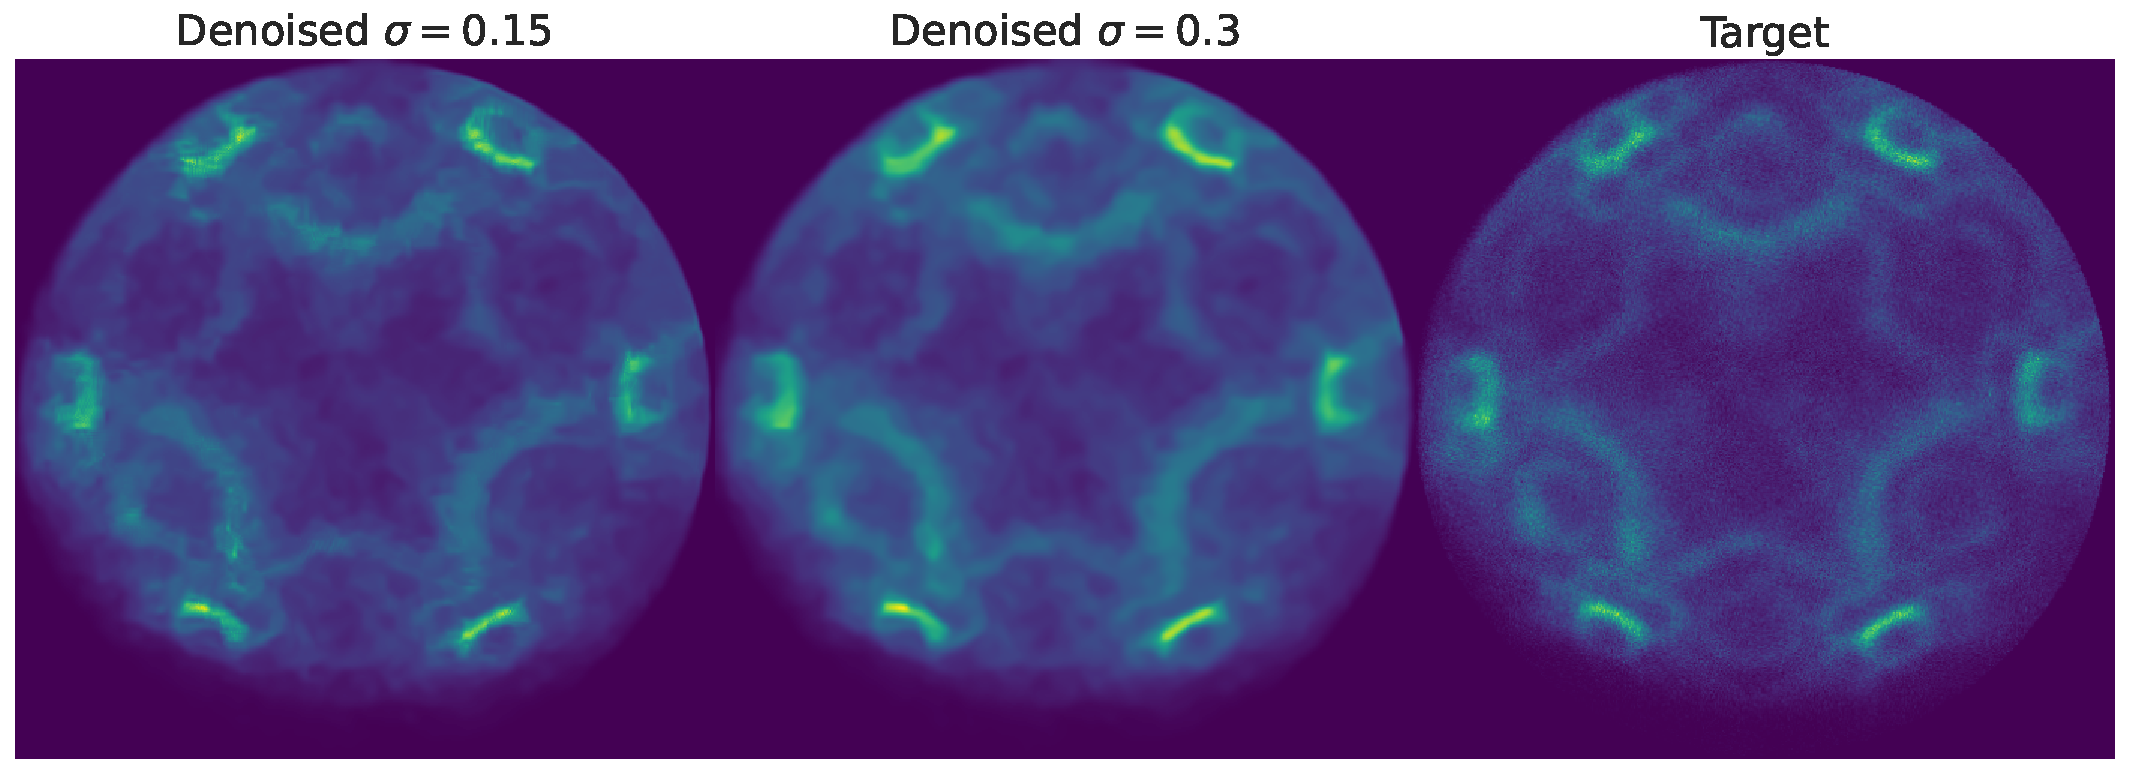
\includegraphics[width=1\linewidth]{images/denoised_optimal_sigma.pdf}
    \caption{Denoised image using the optimal $\sigma_{\text{oo}}=0.15$ (optimal value found for \num{1.6e7} counts from the hyperparameter search) denoised image with $\sigma_{\text{o}}=0.3$ (adjusted optimal value) and the target image.}
    \label{fig:denoised-optimal-sigma}
\end{figure}
Till now, we only looked at a single count rate and denoising with a single $\sigma$ value. However, considering that the noise decreases with increased electron counts, the expectation would be that the level of denoising required also decreases. One way would be to estimate the noise level and use that estimate as the $\sigma$ for denoising. A different approach would be to perform a constrained optimization to find optimal $\sigma$ denoted $\sigma_{\text{oo}}$, such that the metric \gls{MSSSIM} is maximized. For user defined parameters to an algorithm, this sort of optimization is known as a hyperparameter search. An exhaustive grid search is the simplest method, but it is computationally expensive. Therefore, we use \texttt{optuna}\footnote{\href{https://optuna.org/}{https://optuna.org/} see citation in acknowledgments.}, which performs Bayesian optimization to find the optimal parameters, optimizing for \num{50} trials. The search is performed on \num{10} window-averaged 2D image slices (same as in \cref{fig:noisy-denoised-ref-16M-avg-bm3d}) with 5 different noisy realizations for each count.

\begin{figure}
    \centering
    % First subfigure (Hyperparameter Search with Averaged 10 Images using MS-SSIM)
    \begin{subfigure}[t]{0.49\linewidth}
        \centering
        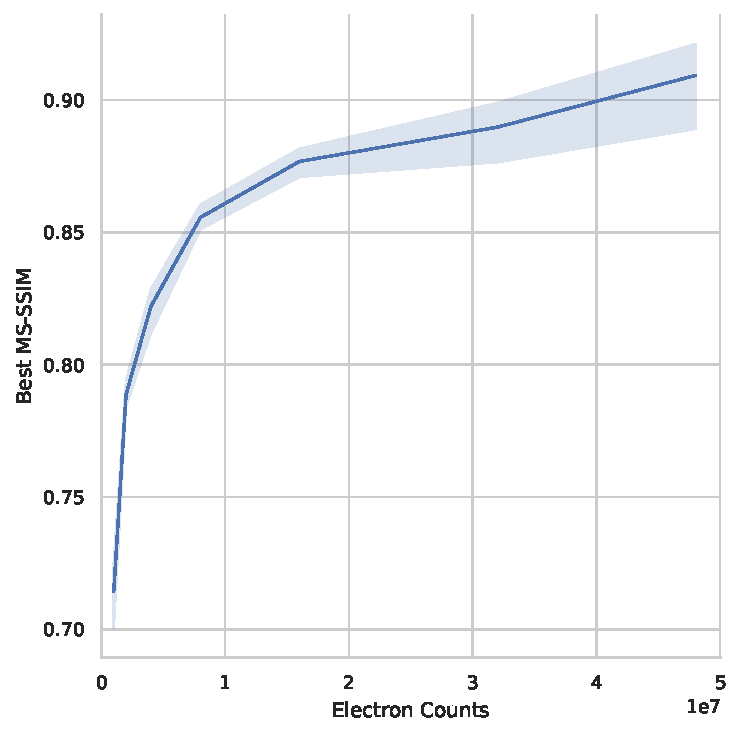
\includegraphics[width=\linewidth]{images/hyperparameter_msssim_averaged_10_images.pdf}
        \caption{Hyperparameter search results using MS-SSIM metric, averaged over 10 images.}
        \label{fig:hyperparameter-msssim-averaged-10-images}
    \end{subfigure}
    \hfill
    % Second subfigure (Hyperparameter Search with Averaged 10 Images using Sigma)
    \begin{subfigure}[t]{0.49\linewidth}
        \centering
        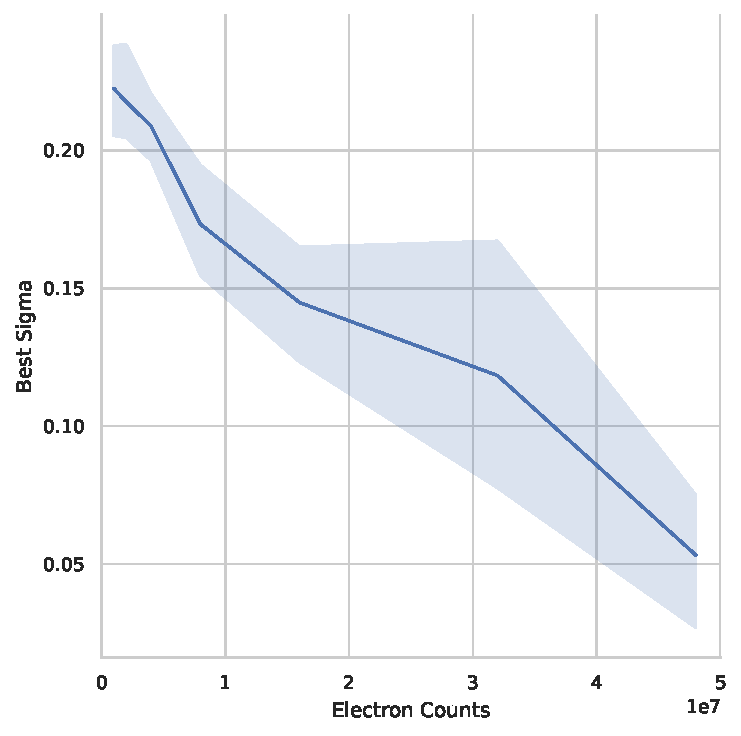
\includegraphics[width=\linewidth]{images/hyperparameter_sigma_averaged_10_images.pdf}
        \caption{Hyperparameter search results using Sigma metric, averaged over 10 images.}
        \label{fig:hyperparameter-sigma-averaged-10-images}
    \end{subfigure}
    \caption{Results of hyperparameter search for \gls{BM3D} $\sigma$ for different electron counts, using the \gls{MSSSIM} metric. The images are a window-average of \num{10} slices from the 3D volume.}
    \label{fig:hyperparameter-averaged-10-images}
\end{figure}

The results in \cref{fig:hyperparameter-averaged-10-images} corroborate the hypothesis that the optimal $\sigma$ for denoising decreases with increasing electron counts, a linearly decreasing trend.

While using \gls{MSSSIM} as the objective function for optimization is good at showing the denoising performance improvement, it leads to more cautious results (low $\sigma_{\text{oo}}$ values) as those fare better against the target, which has the relevant features but is also noisy. To counter that, we scale the optimum $\sigma_{\text{oo}}$ values by a factor of 2 to get a more aggressive denoising and denote that as $\sigma_{\text{o}}$ and use this for denoising. A comparison of the denoised image using the optimal $\sigma_{\text{o}}$ and the adjusted optimal $\sigma_{\text{oo}}$ is shown in \cref{fig:denoised-optimal-sigma}.

The denoising performance below \num{4e6} is poor, with or without the optimal value $\sigma_{\text{oo}}$, even though the \gls{MSSSIM} reports high values. \cref{fig:noisy-denoised-ref-2M-avg-bm3d} and \cref{fig:noisy-denoised-ref-4M-avg-bm3d} show the denoised images for \num{2e6} and \num{4e6} counts, with an average count of \num{0.14} and \num{0.27} in the noisy image, respectively, whereas the average count in target image is \num{12.9}. It can be seen that the perpetual quality of the denoised images is poor, with the features not being well-preserved. This highlights that \gls{BM3D} is not well suited for denoising such low count images.

\subsection{Denoising with Varied Counts}
We now evaluate the denoising performance of \cref{alg:anscombe-bm3d} (\gls{BM3D} with Anscombe) and \cref{alg:bm3d} (\gls{BM3D} without Anscombe), using the optimal $\sigma_{\text{o}}$ values determined through the hyperparameter search. A total of \num{1847} images were extracted from two datasets, each with counts of \numlist{1e6;2e6;4e6;8e6;1.6e7;3.2e7;4.8e7}. These images are window-averaged over 10 slices for both the noisy and target images. 

As before, the \gls{MSSSIM} metric is used, with the baseline computed using the noisy images. Averaging over the large amount of images at varied counts gives us a robust estimate of the denoising performance. Using statistical bootstrapping, where the estimate is computed over multiple resamples of the data, we can also estimate the 95\% confidence interval of the \gls{MSSSIM} metric.

As shown in \cref{fig:bm3d-msssim}, there is a noticeable improvement in image quality with counts up to \num{4e7}, with \gls{MSSSIM} values increasing from \num{0.6} to \num{0.83}. Beyond this count, the metric starts reporting lower values for denoised results, and visual inspection reveals that the denoised images contain similar information as the target, just smoother with preserved features. We can see this in \cref{fig:noisy-denoised-ref-48M-avg-bm3d}, where the denoised image has a lower \gls{MSSSIM} value compared to the noisy image, but the features are well-preserved.

\begin{figure}
    \centering
    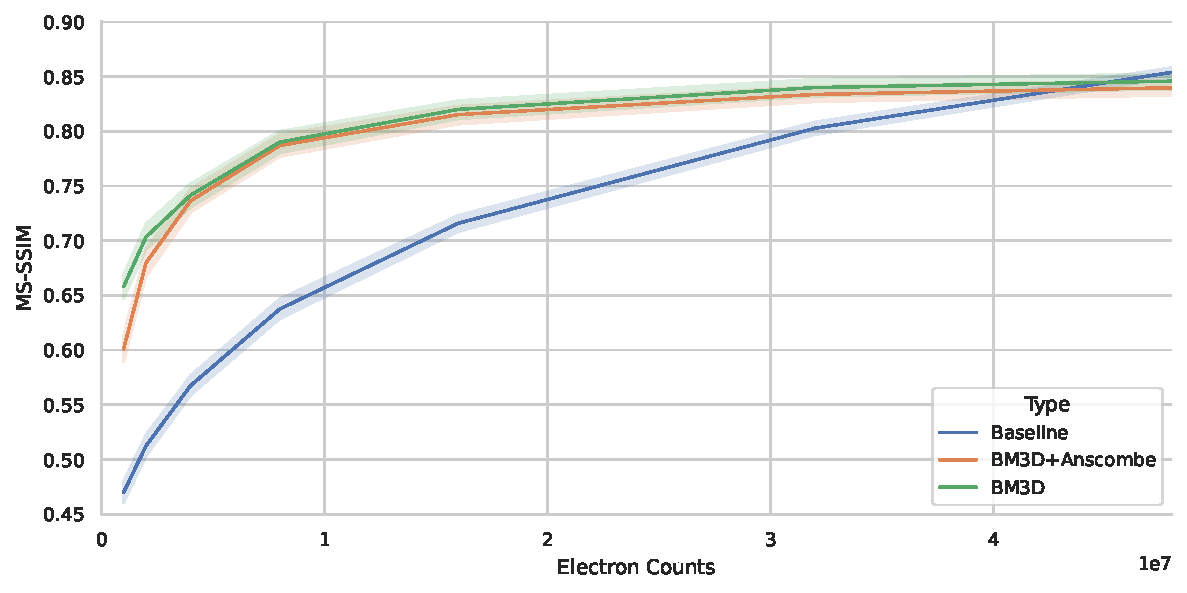
\includegraphics[width=1\linewidth]{images/bm3d_msssim.pdf}
    \caption{Denoising performance of the \gls{BM3D} algorithm, with and without the Anscombe transformation. The optimal $\sigma_{\text{o}}$ values determined through the hyperparameter search are used. The images are window-averages of 10 slices for both the noisy and target images. The baseline metric is computed using the noisy image.}
    \label{fig:bm3d-msssim}
\end{figure}


The most interesting of these results is that applying the \gls{VST} actually leads to a slightly worse performance (\cref{fig:bm3d-msssim} orange vs. green lines), when in fact the expectation on Poissonian noise is that it should improve the denoising performance. This strongly implies that the noise statistics in the image are not Poissonian, as \citeauthor{makitaloOptimalInversionAnscombe2011} have previously demonstrated an improvement in denoising performance using the Anscombe transform on Poissonian noise.
